\section{Producto punto en $\r^n$}

\subsection{}

{\nologo
\begin{frame}\frametitle{Longitud de un vector en $\r^n$}

\begin{center}
	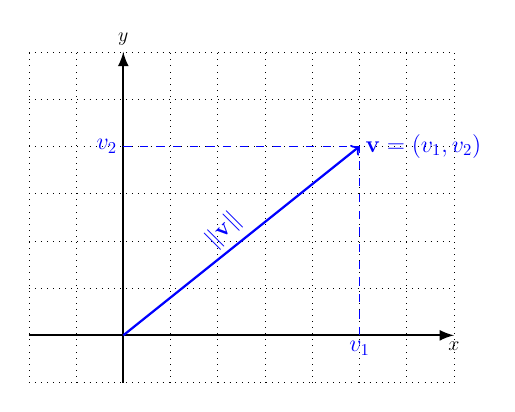
\begin{tikzpicture}[thick,scale=0.6, every node/.style={scale=0.6}]%[scale=.8,font=\scriptsize]
	\draw[help lines,black,dotted] (-2,-1) grid (7,6);
	\draw[thick,-latex] (-2,0) -- (7,0) node[below] {\large $x$};
	\draw[thick,-latex] (0,-1) -- (0,6) node[above] {\large $y$};
	%	\fill[color=green,draw] (0,0) circle (2pt); % node[below, left] {$(0,0)$};
	%	\fill[color=red,draw] (2,3) circle (2pt) node[above, right] {$(x_1,x_2)$};	
	%	\foreach \x in {-4,-3,-2,-1}{\draw[thick] (\x,.1)--(\x,-.1) node[below] {$\x$};}
	%	\foreach \x in {1,2,3,4}{\draw[thick] (\x,.1)--(\x,-.1) node[below] {$\x$};}
	%	\foreach \x in {1,2,3}{\draw[thick] (-.1,\x)--(.1,\x) node[right] {$\x$};}
	%	\foreach \x in {-1,-2,-3}{\draw[thick] (.1,\x)--(-.1,\x) node[left] {$\x$};}
	%	\node at (4.5,3.5) {\Large I}; \node at (-4.5,3.5) {\Large II}; 
	%	\node at (-4.5,-3.5) {\Large III}; \node at (4.5,-3.5) {\Large IV};
	\draw [color=blue,->] (0,0) -- (5,4);
	\fill[color=blue,draw] (5,4) node[above, right] {\Large $\mathbf{v}=(v_1,v_2)$};
%	\draw [color=red,->] (0,0) -- (1,0);
%	\fill[color=red,draw] (1,0) node[below] {$\mathbf{v}_1$};
%	\draw [color=red,->] (0,0) -- (1,2);
%	\draw [color=gray,->] (1,0) -- (7,0);
%	\fill[color=gray,draw] (7,0) node[below] {\large $x'$};
%	\fill[color=red,draw] (1,2) node[above, right] {$\mathbf{v}_2$};
%	\draw [color=gray,->] (1,2) -- (3,6);
%	\fill[color=gray,draw] (3,6) node[above, right] {\large $y'$};
	\draw [line width=0.1mm,color=blue,dashed,-] (5,0) -- (5,4);
	\fill[color=blue,draw] (5,0) node[below] {\Large $v_1$};
	\draw [line width=0.1mm,color=blue,dashed,-] (0,4) -- (5,4);	
	\fill[color=blue,draw] (0,4) node[left] {\Large $v_2$};
	\fill[color=blue,draw] (2.5,2.6) node[rotate=45,left] {\Large $\Vert \mathbf{v}\Vert$};
	\end{tikzpicture}
\end{center}

\begin{defi}{\textbf{Definición 1}}\justifying
	La \textbf{\textit{longitud}} o \textbf{\textit{magnitud}} de un vector $\mathbf{v}=(v_1,\hdots,v_n)$ en $\r^n$ se define como
	\[
		\Vert \mathbf{v}\Vert = \sqrt{v_1^2+v_2^2+\cdots+v_n^2}.
	\]
\end{defi}	

\end{frame}
}

%%------------------------------------------------------------------------------------------------------

\subsection{}

\begin{frame}\frametitle{Longitud de un vector en $\r^n$}

\begin{defi}{\textbf{Definición 1}}\justifying
	La \textbf{\textit{longitud}} o \textbf{\textit{magnitud}} de un vector $\mathbf{v}=(v_1,\hdots,v_n)$ en $\r^n$ se define
	como
	\[
	\Vert \mathbf{v}\Vert = \sqrt{v_1^2+v_2^2+\cdots+v_n^2}.
	\]
\end{defi}	

\begin{ej}{\textbf{Ejemplo 1}}
	\begin{enumerate}\justifying
		\item[\labelname{$a$}] Halle la longitud del vector $\mathbf{v}=(0,-2,1,4,-2)$ de $\r^5$. 
%		\item[\labelname{$b$}] En  $\r^3$, halle la longitud del vector 
%		\[
%			\mathbf{v} = \left( \frac{2}{\sqrt{17}} , -\frac{2}{\sqrt{17}}\,, \frac{3}{\sqrt{17}} \right). 
%		\]
%		\item[\labelname{$c$}] En  $\r^3$, halle la longitud de cada uno de los vectores de la base canónica (estándar)
%		\[
%			\{ (1,0,0), (0,1,0), (0,0,1) \}.
%		\]
	\end{enumerate}
\end{ej}
\textit{Solución}.

\end{frame}

%%------------------------------------------------------------------------------------------------------

\subsection{}

\begin{frame}\frametitle{Longitud de un vector en $\r^n$}
	
	\begin{defi}{\textbf{Definición 1}}\justifying
		La \textbf{\textit{longitud}} o \textbf{\textit{magnitud}} de un vector $\mathbf{v}=(v_1,\hdots,v_n)$ en $\r^n$ se define
		como
		\[
		\Vert \mathbf{v}\Vert = \sqrt{v_1^2+v_2^2+\cdots+v_n^2}.
		\]
	\end{defi}	
	
	\begin{ej}{\textbf{Ejemplo 1}}
		\begin{enumerate}\justifying
%			\item[\labelname{$a$}] Halle la longitud del vector $\mathbf{v}=(0,-2,1,4,-2)$ de $\r^5$. 
			\item[\labelname{$b$}] En  $\r^3$, halle la longitud del vector 
			\[
			\mathbf{v} = \left( \frac{2}{\sqrt{17}} , -\frac{2}{\sqrt{17}}\,, \frac{3}{\sqrt{17}} \right). 
			\]
%			\item[\labelname{$c$}] En  $\r^3$, halle la longitud de cada uno de los vectores de la base canónica (estándar)
%			\[
%			\{ (1,0,0), (0,1,0), (0,0,1) \}.
%			\]
		\end{enumerate}
	\end{ej}
	\textit{Solución}.
	
\end{frame}

%%------------------------------------------------------------------------------------------------------

\subsection{}

\begin{frame}\frametitle{Longitud de un vector en $\r^n$}
	
	\begin{defi}{\textbf{Definición 1}}\justifying
		La \textbf{\textit{longitud}} o \textbf{\textit{magnitud}} de un vector $\mathbf{v}=(v_1,\hdots,v_n)$ en $\r^n$ se define
		como
		\[
		\Vert \mathbf{v}\Vert = \sqrt{v_1^2+v_2^2+\cdots+v_n^2}.
		\]
	\end{defi}	
	
	\begin{ej}{\textbf{Ejemplo 1}}
		\begin{enumerate}\justifying
%			\item[\labelname{$a$}] Halle la longitud del vector $\mathbf{v}=(0,-2,1,4,-2)$ de $\r^5$. 
%			\item[\labelname{$b$}] En  $\r^3$, halle la longitud del vector 
%			\[
%			\mathbf{v} = \left( \frac{2}{\sqrt{17}} , -\frac{2}{\sqrt{17}}\,, \frac{3}{\sqrt{17}} \right). 
%			\]
			\item[\labelname{$c$}] En  $\r^3$, halle la longitud de cada uno de los vectores de la base canónica (estándar)
			\[
			\{ (1,0,0), (0,1,0), (0,0,1) \}.
			\]
		\end{enumerate}
	\end{ej}
	\textit{Solución}.
	
\end{frame}

%%------------------------------------------------------------------------------------------------------

\subsection{}

\begin{frame}\frametitle{Vectores unitarios}
	
	\begin{prop}{\textbf{Propiedad 1}}
		\justifying
		Si $\mathbf{v}$ es un vector en $\r^n$ y $c$ es un escalar, entonces
		\[
		\Vert c\mathbf{v}\Vert = |c| \Vert \mathbf{v}\Vert
		\]
	\end{prop}	
	
	\begin{prop}{\textbf{Propiedad 2}}
		\justifying
		Si $\mathbf{v}$ es un vector en $\r^n$ diferente del vector cero, entonces
		\[
		\mathbf{u} = \frac{\mathbf{v}}{\Vert \mathbf{v}\Vert} 
		\]
		es un vector de longitud 1 (\textbf{\textit{vector unitario}}) en la dirección de $\mathbf{v}$.
	\end{prop}	
	
%	\begin{ej}{\textbf{Ejemplo 2}}
%		Encuentre el vector unitario en la dirección del vector $\mathbf{v}=(3,-1,2)$.
%	\end{ej}
	
\end{frame}

%%------------------------------------------------------------------------------------------------------

\subsection{}

\begin{frame}\frametitle{Vectores unitarios}

%\begin{prop}{\textbf{Propiedad 1}}
%	\justifying
%	Si $\mathbf{v}$ es un vector en $\r^n$ y $c$ es un escalar, entonces
%	\[
%		\Vert c\mathbf{v}\Vert = |c| \Vert \mathbf{v}\Vert
%	\]
%\end{prop}	

\begin{prop}{\textbf{Propiedad 2}}
	\justifying
	Si $\mathbf{v}$ es un vector en $\r^n$ diferente del vector cero, entonces
	\[
		\mathbf{u} = \frac{\mathbf{v}}{\Vert \mathbf{v}\Vert} 
	\]
	es un vector de longitud 1 (\textbf{\textit{vector unitario}}) en la dirección de $\mathbf{v}$.
\end{prop}	

\begin{ej}{\textbf{Ejemplo 2}}
	Encuentre el vector unitario en la dirección del vector $\mathbf{v}=(3,-1,2)$.
\end{ej}
\textit{Solución}.

\end{frame}

%%------------------------------------------------------------------------------------------------------

\subsection{}

{\nologo
\begin{frame}\frametitle{Distancia entre dos vectores de $\r^n$}

\begin{center}
	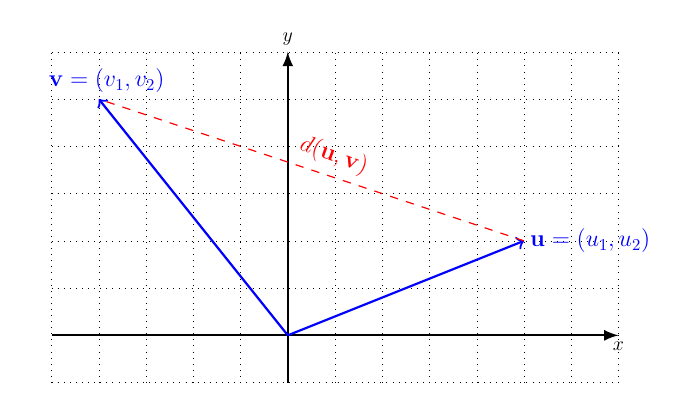
\begin{tikzpicture}[thick,scale=0.6, every node/.style={scale=0.6}]%[scale=.8,font=\scriptsize]
	\draw[help lines,black,dotted] (-5,-1) grid (7,6);
	\draw[thick,-latex] (-5,0) -- (7,0) node[below] {\large $x$};
	\draw[thick,-latex] (0,-1) -- (0,6) node[above] {\large $y$};	
	% vector u
	\draw [color=blue,->] (0,0) -- (5,2);
	\fill[color=blue,draw] (5,2) node[above, right] {\Large $\mathbf{u}=(u_1,u_2)$};
%	\draw [line width=0.1mm,color=blue,dashed,-] (5,0) -- (5,2);
%	\fill[color=blue,draw] (5,0) node[below] {\Large $v_1$};
%	\draw [line width=0.1mm,color=blue,dashed,-] (0,2) -- (5,2);	
%	\fill[color=blue,draw] (0,2) node[left] {\Large $v_2$};
	% vector v
	\draw [color=blue,->] (0,0) -- (-4,5);
	\fill[color=blue,draw] (-4,5) node[above] {\Large \ \  $\mathbf{v}=(v_1,v_2)$};
	\draw [line width=0.15mm,color=red,dashed,-] (5,2) -- (-4,5);	
	\fill[color=red,draw] (1.8,3.5) node[rotate=-20,left] {\Large $d(\mathbf{u}, \mathbf{v})$};
	\end{tikzpicture}
\end{center}

\begin{defi}{\textbf{Definición 2}}\justifying
	La \textbf{\textit{distancia}} entre dos vectores $\mathbf{u}$ y $\mathbf{v}$ de $\r^n$ se define como
	\[
	d(\mathbf{u},\mathbf{v}) = \Vert \mathbf{v} - \mathbf{u}\Vert = \sqrt{\left(v_1-u_1 \right)^2+\cdots+\left(v_n-u_n \right)^2}.
	\]
\end{defi}	

\end{frame}
}

%%------------------------------------------------------------------------------------------------------

\subsection{}

\begin{frame}\frametitle{Distancia entre dos vectores de $\r^n$}
	
	\begin{defi}{\textbf{Definición 2}}\justifying
		La \textbf{\textit{distancia}} entre dos vectores $\mathbf{u}$ y $\mathbf{v}$ de $\r^n$ se define como
		\[
		d(\mathbf{u},\mathbf{v}) = \Vert \mathbf{v} - \mathbf{u}\Vert = \sqrt{\left(v_1-u_1 \right)^2+\cdots+\left(v_n-u_n \right)^2}.
		\]
	\end{defi}	
	
	\begin{ej}{\textbf{Ejemplo 3}}
		Encuentre la distancia entre los vectores de  $\r^3$
		\[
		\mathbf{u}=(0,0,2) \qquad \text{y} \qquad \mathbf{v}=(2,0,1).
		\]
	\end{ej}
	\textit{Solución}.
	
\end{frame}

%%------------------------------------------------------------------------------------------------------

\subsection{}

{\nologo
\begin{frame}\frametitle{Distancia entre dos vectores de $\r^n$}

\vspace{-2mm}

\begin{center}
	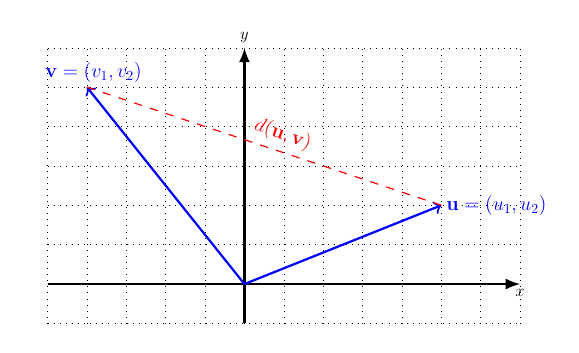
\begin{tikzpicture}[thick,scale=0.5, every node/.style={scale=0.5}]%[scale=.8,font=\scriptsize]
	\draw[help lines,black,dotted] (-5,-1) grid (7,6);
	\draw[thick,-latex] (-5,0) -- (7,0) node[below] {\large $x$};
	\draw[thick,-latex] (0,-1) -- (0,6) node[above] {\large $y$};	
	% vector u
	\draw [color=blue,->] (0,0) -- (5,2);
	\fill[color=blue,draw] (5,2) node[above, right] {\Large $\mathbf{u}=(u_1,u_2)$};
	%	\draw [line width=0.1mm,color=blue,dashed,-] (5,0) -- (5,2);
	%	\fill[color=blue,draw] (5,0) node[below] {\Large $v_1$};
	%	\draw [line width=0.1mm,color=blue,dashed,-] (0,2) -- (5,2);	
	%	\fill[color=blue,draw] (0,2) node[left] {\Large $v_2$};
	% vector v
	\draw [color=blue,->] (0,0) -- (-4,5);
	\fill[color=blue,draw] (-4,5) node[above] {\Large \ \  $\mathbf{v}=(v_1,v_2)$};
	\draw [line width=0.15mm,color=red,dashed,-] (5,2) -- (-4,5);	
	\fill[color=red,draw] (1.8,3.5) node[rotate=-20,left] {\Large $d(\mathbf{u}, \mathbf{v})$};
	\end{tikzpicture}
\end{center}

\vspace{-1mm}

\begin{prop}{\textbf{Propiedad 3}}
	\justifying
	La distancia entre vectores de $\r^n$,
	\[
		d(\mathbf{u},\mathbf{v}) = \Vert \mathbf{v} - \mathbf{u}\Vert
	\]
	satisface las siguientes propiedades:
	
	\vspace{-2mm}
	\begin{multicols}{2}
		\begin{enumerate}
			\item[\labelname{$a$}] $d(\mathbf{u},\mathbf{v}) \geq 0$. \\[2mm]
			\item[\labelname{$b$}] $d(\mathbf{u},\mathbf{v}) = 0$ si y sólo si $\mathbf{u}=\mathbf{v}$.\\[0mm]
			\item[\labelname{$c$}] $d(\mathbf{u},\mathbf{v}) = d(\mathbf{v},\mathbf{u})$.
			\item[]
		\end{enumerate}
	\end{multicols}
\end{prop}	

\end{frame}
}

%%------------------------------------------------------------------------------------------------------

\subsection{}

{\nologo
\begin{frame}\frametitle{Ángulo entre dos vectores de $\r^2$}

\begin{center}
	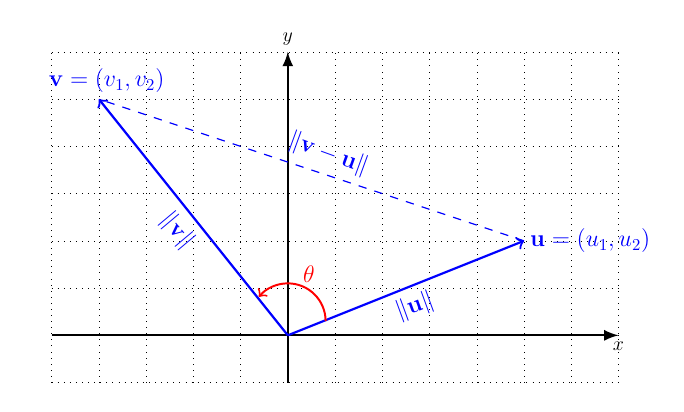
\begin{tikzpicture}[thick,scale=0.6, every node/.style={scale=0.6}]%[scale=.8,font=\scriptsize]
	\draw[help lines,black,dotted] (-5,-1) grid (7,6);
	\draw[thick,-latex] (-5,0) -- (7,0) node[below] {\large $x$};
	\draw[thick,-latex] (0,-1) -- (0,6) node[above] {\large $y$};	
	% vector u
	\draw [color=blue,->] (0,0) -- (5,2);
	\fill[color=blue,draw] (5,2) node[above, right] {\Large $\mathbf{u}=(u_1,u_2)$};
	\fill[color=blue,draw] (3.2,0.8) node[rotate=20,left] {\Large $\Vert \mathbf{u}\Vert $};
	%	\draw [line width=0.1mm,color=blue,dashed,-] (5,0) -- (5,2);
	%	\fill[color=blue,draw] (5,0) node[below] {\Large $v_1$};
	%	\draw [line width=0.1mm,color=blue,dashed,-] (0,2) -- (5,2);	
	%	\fill[color=blue,draw] (0,2) node[left] {\Large $v_2$};
	% vector v
	\draw [color=blue,->] (0,0) -- (-4,5);
	\fill[color=blue,draw] (-4,5) node[above] {\Large \ \  $\mathbf{v}=(v_1,v_2)$};
	\draw [line width=0.15mm,color=blue,dashed,-] (5,2) -- (-4,5);	
	\fill[color=blue,draw] (-2,1.8) node[rotate=-50,left] {\Large $\Vert \mathbf{v}\Vert $};
	\fill[color=blue,draw] (1.8,3.5) node[rotate=-20,left] {\Large $ \Vert \mathbf{v} - \mathbf{u} \Vert$};
	% https://tex.stackexchange.com/a/175027
	\draw[line width=0.25mm,red,->] (0.8,0.3) arc (0:140:0.8);
	\fill[color=red,draw] (0.7,1.3) node[left] {\Large $\theta$};
	\end{tikzpicture}
\end{center}

\begin{prop}{\textbf{Propiedad 4}}
	\justifying
	El ángulo $\theta$ $(0\leq \theta\leq \pi)$ entre dos vectores no nulos $\mathbf{u}=(u_1,u_2)$ y $\mathbf{v}=(v_1,v_2)$ del 
	plano, está dado por
	
	\vspace{-2mm}
	\[
	 \cos\theta = \frac{u_1v_1+u_2v_2}{\Vert \mathbf{u}\Vert \, \Vert \mathbf{v}\Vert} 
	\]
\end{prop}	

\end{frame}
}

%%------------------------------------------------------------------------------------------------------

\subsection{}

\begin{frame}\frametitle{Producto escalar (o punto) en $\r^n$}
	
	\begin{defi}{\textbf{Definición 3}}\justifying
		Recordemos que el \textbf{\textit{producto punto}} o \textbf{\textit{producto escalar}} de dos vectores
		\[
		\mathbf{u}=(u_1,\hdots,u_n) \qquad \text{y} \qquad \mathbf{v}=(v_1,\hdots,v_n)
		\]
		de $\r^n$ se define como
		\[
		\mathbf{u} \cdot \mathbf{v} = u_1 v_1 + u_2 v_2 +  \cdots + u_n v_n.
		\]
	\end{defi}	
	
	\vspace{0mm}
	
	\begin{alertblock}{\textbf{Observación 1}}
		El producto punto $\mathbf{u} \cdot \mathbf{v}$ de dos vectores es un escalar y \textbf{\textit{no}} un vector.
	\end{alertblock}
	
%	\begin{ej}{\textbf{Ejemplo 4}}
%		Encuentre el producto escalar de los vectores 
%		\[
%		\mathbf{u}=(1,2,0,-3) \qquad \text{y} \qquad \mathbf{v}=(3,-2,4,2).
%		\]
%	\end{ej}
	
\end{frame}


%%------------------------------------------------------------------------------------------------------

\subsection{}

\begin{frame}\frametitle{Producto escalar (o punto) en $\r^n$}

\begin{defi}{\textbf{Definición 3}}\justifying
	Recordemos que el \textbf{\textit{producto punto}} o \textbf{\textit{producto escalar}} de dos vectores
	\[
		\mathbf{u}=(u_1,\hdots,u_n) \qquad \text{y} \qquad \mathbf{v}=(v_1,\hdots,v_n)
	\]
	de $\r^n$ se define como
	\[
	\mathbf{u} \cdot \mathbf{v} = u_1 v_1 + u_2 v_2 +  \cdots + u_n v_n.
	\]
\end{defi}	

\vspace{0mm}

%\begin{alertblock}{\textbf{Observación 1}}
%	El producto punto $\mathbf{u} \cdot \mathbf{v}$ de dos vectores es un escalar y \textbf{\textit{no}} un vector.
%\end{alertblock}

\begin{ej}{\textbf{Ejemplo 4}}
	Encuentre el producto escalar de los vectores 
	\[
		\mathbf{u}=(1,2,0,-3) \qquad \text{y} \qquad \mathbf{v}=(3,-2,4,2).
	\]
\end{ej}
\textit{Solución}.

\end{frame}

%%------------------------------------------------------------------------------------------------------

\subsection{}

\begin{frame}\frametitle{Propiedades del producto escalar}
	
	\begin{prop}{\textbf{Propiedad 5}}
		\justifying
		Si $\mathbf{u}, \mathbf{v}$ y $\mathbf{w}$ son vectores en $\r^n$ y $c$ es un escalar, entonces se satisfacen 
		las siguientes propiedades:
		\begin{enumerate}
			\item[\labelname{$a$}] $\mathbf{u}\cdot \mathbf{v} = \mathbf{v}\cdot \mathbf{u}$
			\item[\labelname{$b$}] $\mathbf{u}\cdot (\mathbf{v}+\mathbf{w}) = \mathbf{u}\cdot \mathbf{v} + \mathbf{u}\cdot \mathbf{w}$
			\item[\labelname{$c$}] $c(\mathbf{u}\cdot \mathbf{v}) = (c\mathbf{u})\cdot \mathbf{v} = \mathbf{u}\cdot (c\mathbf{v})$
			\item[\labelname{$d$}] $\mathbf{v}\cdot \mathbf{v} = \Vert \mathbf{v} \Vert^2$
			\item[\labelname{$e$}] $\mathbf{v}\cdot \mathbf{v} \geq 0$
			\item[\labelname{$e$}] $\mathbf{v}\cdot \mathbf{v} = 0$ si y sólo si $\mathbf{v} = \mathbf{0}$
		\end{enumerate}
	\end{prop}	
	
	

\end{frame}

%%------------------------------------------------------------------------------------------------------

\subsection{}

\begin{frame}\frametitle{Propiedades del producto escalar}

\begin{ej}{\textbf{Ejemplo 5}}
	Considere los vectores
	
	\vspace{-2mm}
	\[
		\mathbf{u}=(2,-2), \qquad \mathbf{v}=(5,8), \qquad \text{y} \qquad \mathbf{w}=(-4,3).
	\]
	
	\vspace{-1mm}
	Calcule
	
	\vspace{-2mm}
	\begin{multicols}{3}
		\begin{enumerate}
			\item[\labelname{$a$}] $\mathbf{u}\cdot \mathbf{v}$
			\item[\labelname{$b$}] $(\mathbf{u}\cdot \mathbf{v}) \mathbf{w}$
			\item[\labelname{$c$}] $\mathbf{u}\cdot (2\mathbf{v})$
			\item[\labelname{$d$}] $\Vert \mathbf{w} \Vert^2$
			\item[\labelname{$e$}] $\mathbf{u}\cdot (\mathbf{v}-2\mathbf{w})$
			\item[]
		\end{enumerate}
	\end{multicols}
\end{ej}
\textit{Solución}.

\end{frame}

%%------------------------------------------------------------------------------------------------------

\subsection{}

\begin{frame}\frametitle{Ángulo entre vectores de $\r^n$}
	
	\begin{prop}{\textbf{Propiedad 6 (Desigualdad de Cauchy-Schwarz)}}
		\justifying
		Si $\mathbf{u}$ y $\mathbf{v}$ son vectores de $\r^n$, entonces
		\[
		|\mathbf{u}\cdot \mathbf{v}| \leq \Vert \mathbf{u}\Vert\ \Vert \mathbf{v}\Vert,
		\]
		donde $|\mathbf{u}\cdot \mathbf{v}|$ denota el valor absoluto del producto escalar $\mathbf{u}\cdot \mathbf{v}$.
	\end{prop}	
	
	\vspace{0mm}
	
	\begin{defi}{\textbf{Definición 4}}\justifying
		\justifying
		El ángulo $\theta$ entre dos vectores no nulos $\mathbf{u}$ y $\mathbf{v}$ de $\r^n$ 
		está dado por
		
		\vspace{-0mm}
		\[
		\cos\theta = \frac{\mathbf{u}\cdot \mathbf{v}}{\Vert \mathbf{u}\Vert \, \Vert \mathbf{v}\Vert} , \qquad 0\leq \theta\leq \pi.
		\]
	\end{defi}	
	
	
\end{frame}


%%------------------------------------------------------------------------------------------------------

\subsection{}

\begin{frame}\frametitle{Ángulo entre vectores de $\r^n$}

\begin{defi}{\textbf{Definición 4}}\justifying
	\justifying
	El ángulo $\theta$ entre dos vectores no nulos $\mathbf{u}$ y $\mathbf{v}$ de $\r^n$ 
	está dado por
	
	\vspace{-0mm}
	\[
	\cos\theta = \frac{\mathbf{u}\cdot \mathbf{v}}{\Vert \mathbf{u}\Vert \, \Vert \mathbf{v}\Vert} , \qquad 0\leq \theta\leq \pi.
	\]
\end{defi}	

\begin{ej}{\textbf{Ejemplo 6}}
	Calcule el ángulo entre los vectores
	\[
	\mathbf{u}=(-4,0,2,-2)  \qquad \text{y} \qquad \mathbf{v}=(2,0,-1,1).
	\]
\end{ej}
\textit{Solución}.

\end{frame}

%%------------------------------------------------------------------------------------------------------

\subsection{}

\begin{frame}\frametitle{Ángulo entre vectores de $\r^n$}

\begin{defi}{\textbf{Definición 4}}\justifying
	\justifying
	El ángulo $\theta$ entre dos vectores no nulos $\mathbf{u}$ y $\mathbf{v}$ de $\r^n$ 
	está dado por
	
	\vspace{-0mm}
	\[
	\cos\theta = \frac{\mathbf{u}\cdot \mathbf{v}}{\Vert \mathbf{u}\Vert \, \Vert \mathbf{v}\Vert} , \qquad 0\leq \theta\leq \pi.
	\]
\end{defi}	

\begin{alertblock}{\textbf{Observación 2}}\justifying
	En la definición 4, $\Vert \mathbf{u}\Vert$ y $\Vert \mathbf{v}\Vert$ siempre son positivos y por tanto
	
	\vspace{-2mm}
	\begin{multicols}{2}
		\begin{enumerate}
			\item[\labelname{$a$}] $\cos\theta$ y $\mathbf{u}\cdot \mathbf{v}$ son positivos ó
			\item[\labelname{$b$}] $\cos\theta$ y $\mathbf{u}\cdot \mathbf{v}$ son negativos.\\
		\end{enumerate}
	\end{multicols}

\end{alertblock}

\vspace{-2mm}

\begin{figure}	
	\begin{subfigure}[b]{0.45\textwidth}
		\centering
		\begin{tikzpicture}[thick,scale=0.7, every node/.style={scale=0.6}]%[scale=.8,font=\scriptsize]
		\draw[help lines,white,dotted] (-2,-1) grid (2,2);
		\fill[color=blue] (0,0) circle[radius=2pt];	
		% Vector u
		\draw [line width=0.27mm,color=blue,->] (0,0) -- (2,0);
		\fill[color=blue,draw] (1.8,-0.3) node[below,right] {\Large $\mathbf{u} $};	
		%	\fill[color=red,draw] (0.2,0.8) node[left] {\Large $\theta$};
		% Vector v
		\draw [line width=0.27mm,color=blue,->] (0,0) -- (1.4,0);
		\fill[color=blue,draw] (1.1,-0.3) node[below,right] {\Large $\mathbf{v} $};	
		%	\draw[line width=0.2mm,red,->] (0.5,0) arc (0:180:0.5);
		% Valores del ángulo
		\fill[draw] (0.55,-0.8) node[left] {\Large $\theta=0$};
		\fill[draw] (0.55,-1.3) node[left] {\Large $\cos\theta=1$};
		\end{tikzpicture}
		\caption{Direcciones iguales}
		\label{fig:gull}
	\end{subfigure}
	~ %add desired spacing between images, e. g. ~, \quad, \qquad, \hfill etc. 
	%(or a blank line to force the subfigure onto a new line)
	\begin{subfigure}[b]{0.45\textwidth}
		\centering
		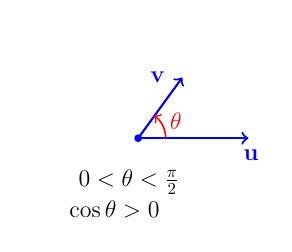
\begin{tikzpicture}[thick,scale=0.7, every node/.style={scale=0.6}]%[scale=.8,font=\scriptsize]
		\draw[help lines,white,dotted] (-2,-1) grid (2,2);
		\fill[color=blue] (0,0) circle[radius=2pt];	
		% Vector u
		\draw [line width=0.27mm,color=blue,->] (0,0) -- (2,0);
		\fill[color=blue,draw] (1.8,-0.3) node[below,right] {\Large $\mathbf{u} $};	
		% Vector v
		\draw [line width=0.27mm,color=blue,->] (0,0) -- (0.8,1.1);
		\fill[color=blue,draw] (0.6,1.1) node[below,left] {\Large $\mathbf{v} $};	
		\draw[line width=0.2mm,red,->] (0.5,0) arc (0:55:0.5);
		\fill[color=red,draw] (0.9,0.3) node[left] {\Large $\theta$};
		% Valores del ángulo
		\fill[draw] (0.85,-0.8) node[left] {\Large $0<\theta<\frac{\pi}{2}$};
		\fill[draw] (0.5,-1.3) node[left] {\Large $\cos\theta>0$};
		\end{tikzpicture}
		\caption{$\mathbf{u}\cdot \mathbf{v}>0$}
		\label{fig:mouse}
	\end{subfigure}
%	\caption{Pictures of animals}\label{fig:animals}
\end{figure}

\end{frame}

%%------------------------------------------------------------------------------------------------------

\subsection{}

\begin{frame}\frametitle{Ángulo entre vectores de $\r^n$}

\begin{defi}{\textbf{Definición 4}}\justifying
	\justifying
	El ángulo $\theta$ entre dos vectores no nulos $\mathbf{u}$ y $\mathbf{v}$ de $\r^n$ 
	está dado por
	
	\vspace{-0mm}
	\[
	\cos\theta = \frac{\mathbf{u}\cdot \mathbf{v}}{\Vert \mathbf{u}\Vert \, \Vert \mathbf{v}\Vert} , \qquad 0\leq \theta\leq \pi.
	\]
\end{defi}	

\begin{alertblock}{\textbf{Observación 2}}\justifying
	En la definición 4, $\Vert \mathbf{u}\Vert$ y $\Vert \mathbf{v}\Vert$ siempre son positivos y por tanto
	
	\vspace{-2mm}
	\begin{multicols}{2}
		\begin{enumerate}
			\item[\labelname{$a$}] $\cos\theta$ y $\mathbf{u}\cdot \mathbf{v}$ son positivos ó
			\item[\labelname{$b$}] $\cos\theta$ y $\mathbf{u}\cdot \mathbf{v}$ son negativos.\\
		\end{enumerate}
	\end{multicols}
	
\end{alertblock}

\vspace{-2mm}

\begin{figure}	
	\begin{subfigure}[b]{0.45\textwidth}
		\centering
		\begin{tikzpicture}[thick,scale=0.7, every node/.style={scale=0.6}]%[scale=.8,font=\scriptsize]
		\draw[help lines,white,dotted] (-2,-1) grid (2,2);
		\fill[color=blue] (0,0) circle[radius=2pt];	
		% Vector u
		\draw [line width=0.27mm,color=blue,->] (0,0) -- (2,0);
		\fill[color=blue,draw] (1.8,-0.3) node[below,right] {\Large $\mathbf{u} $};	
		%	\fill[color=red,draw] (0.2,0.8) node[left] {\Large $\theta$};
		% Vector v
		\draw [line width=0.27mm,color=blue,->] (0,0) -- (0,1.4);
		\fill[color=blue,draw] (0,1.4) node[below,right] {\Large $\mathbf{v} $};	
		\draw [line width=0.26mm,color=red,-] (0.3,0) -- (0.3,0.3) -- (0,0.3);
		%	\draw[line width=0.2mm,red,->] (0.5,0) arc (0:180:0.5);
		% Valores del ángulo
		\fill[draw] (0.55,-0.8) node[left] {\Large $\theta=\frac{\pi}{2}$};
		\fill[draw] (0.5,-1.3) node[left] {\Large $\cos\theta=0$};
		\end{tikzpicture}
		\caption{$\mathbf{u}\cdot \mathbf{v}=0$}
		\label{fig:gull}
	\end{subfigure}
	~ %add desired spacing between images, e. g. ~, \quad, \qquad, \hfill etc. 
	%(or a blank line to force the subfigure onto a new line)
	\begin{subfigure}[b]{0.45\textwidth}
		\centering
		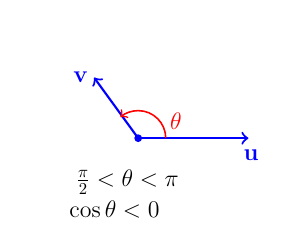
\begin{tikzpicture}[thick,scale=0.7, every node/.style={scale=0.6}]%[scale=.8,font=\scriptsize]
		\draw[help lines,white,dotted] (-2,-1) grid (2,2);
		\fill[color=blue] (0,0) circle[radius=2pt];	
		% Vector u
		\draw [line width=0.27mm,color=blue,->] (0,0) -- (2,0);
		\fill[color=blue,draw] (1.8,-0.3) node[below,right] {\Large $\mathbf{u} $};	
		% Vector v
		\draw [line width=0.27mm,color=blue,->] (0,0) -- (-0.8,1.1);
		\fill[color=blue,draw] (-0.8,1.1) node[below,left] {\Large $\mathbf{v} $};	
		\draw[line width=0.2mm,red,->] (0.5,0) arc (0:130:0.5);
		\fill[color=red,draw] (0.9,0.3) node[left] {\Large $\theta$};
		% Valores del ángulo
		\fill[draw] (0.85,-0.8) node[left] {\Large $\frac{\pi}{2}<\theta<\pi$};
		\fill[draw] (0.5,-1.3) node[left] {\Large $\cos\theta<0$};
		\end{tikzpicture}
		\caption{$\mathbf{u}\cdot \mathbf{v}<0$}
		\label{fig:mouse}
	\end{subfigure}
	%	\caption{Pictures of animals}\label{fig:animals}
\end{figure}

\end{frame}

%%------------------------------------------------------------------------------------------------------

\subsection{}

\begin{frame}\frametitle{Ángulo entre vectores de $\r^n$}
	
	\begin{defi}{\textbf{Definición 5}}\justifying
		\justifying
		Dos vectores $\mathbf{u}$ y $\mathbf{v}$ de $\r^n$ se dice que son \textbf{\textit{ortogonales}} (o \textbf{\textit{perpendiculares}}) si 
		
		\vspace{-5mm}
		\[
		\mathbf{u}\cdot \mathbf{v} = 0.
		\]
	\end{defi}	
	
	\begin{ej}{\textbf{Ejemplo 7}}
		Determine si los siguientes vectores de $\r^3$ son ortogonales.
		\begin{enumerate}
			\item[\labelname{$a$}] $\mathbf{u}=(1,0,0)$ y $\mathbf{v}=(0,0,1)$.
			\item[\labelname{$b$}] $\mathbf{u}=(3,2,-1,4)$ y $\mathbf{v}=(1,-1,1,0)$.
		\end{enumerate}		
	\end{ej}	
	\textit{Solución}.
	
\end{frame}


%%------------------------------------------------------------------------------------------------------

\subsection{}

\begin{frame}\frametitle{Ángulo entre vectores de $\r^n$}

\begin{defi}{\textbf{Definición 5}}\justifying
	\justifying
	Dos vectores $\mathbf{u}$ y $\mathbf{v}$ de $\r^n$ se dice que son \textbf{\textit{ortogonales}} (o \textbf{\textit{perpendiculares}}) si 

	\vspace{-5mm}
	\[
		\mathbf{u}\cdot \mathbf{v} = 0.
	\]
\end{defi}	

\begin{ej}{\textbf{Ejemplo 8}}
	Determine todos los vectores de $\r^2$ que son ortogonales a $\mathbf{u}=(4,2)$.	
\end{ej}
\textit{Solución}.

\end{frame}

%%------------------------------------------------------------------------------------------------------

\subsection{}

{\nologo
\begin{frame}\frametitle{Desigualdad triangular}

\begin{center}
	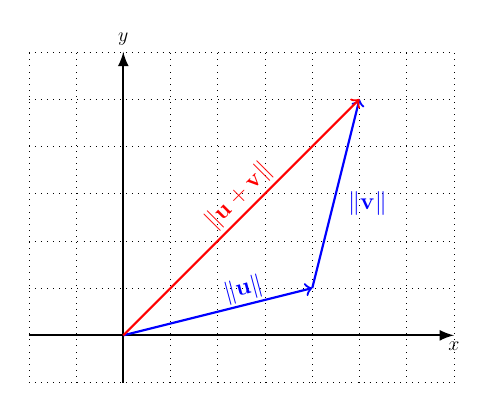
\begin{tikzpicture}[thick,scale=0.6, every node/.style={scale=0.6}]%[scale=.8,font=\scriptsize]
	\draw[help lines,black,dotted] (-2,-1) grid (7,6);
	\draw[thick,-latex] (-2,0) -- (7,0) node[below] {\large $x$};
	\draw[thick,-latex] (0,-1) -- (0,6) node[above] {\large $y$};	
	% vector u
	\draw [color=blue,->] (0,0) -- (4,1);
%	\fill[color=blue,draw] (4,0.5) node[below,left] {\Large $\mathbf{u}$};
	\fill[color=blue,draw] (1.7,0.75) node[rotate=15,right] {\Large \ \  $\Vert\mathbf{u}\Vert$};
	%	\draw [line width=0.1mm,color=blue,dashed,-] (5,0) -- (5,2);
	%	\fill[color=blue,draw] (5,0) node[below] {\Large $v_1$};
	%	\draw [line width=0.1mm,color=blue,dashed,-] (0,2) -- (5,2);	
	%	\fill[color=blue,draw] (0,2) node[left] {\Large $v_2$};
	% vector v
	\draw [color=blue,->] (4,1) -- (5,5);
%	\fill[color=blue,draw] (4.8,4.8) node[right] {\Large \ \  $\mathbf{v}$};
	\fill[color=blue,draw] (4.3,2.8) node[rotate=0,right] {\Large \ \  $\Vert\mathbf{v}\Vert$};
%	\draw [line width=0.15mm,color=red,dashed,-] (5,2) -- (-4,5);	
%	\fill[color=red,draw] (1.8,3.5) node[rotate=-20,left] {\Large $d(\mathbf{u}, \mathbf{v})$};
	% vector u+v
	\draw [color=red,->] (0,0) -- (5,5);	
	\fill[color=red,draw] (1.5,2) node[rotate=45,right] {\Large \ \  $\Vert\mathbf{u}+\mathbf{v}\Vert$};
	\end{tikzpicture}
\end{center}

\begin{prop}{\textbf{Propiedad 7 (Desigualdad triangular)}}
	\justifying
	Si $\mathbf{u}$ y $\mathbf{v}$ son vectores de $\r^n$, entonces
	\[
		\Vert \mathbf{u} + \mathbf{v}\Vert \leq \Vert \mathbf{u}\Vert + \Vert \mathbf{v}\Vert.
	\]
\end{prop}	

\end{frame}
}

%%------------------------------------------------------------------------------------------------------

\subsection{}

{\nologo
\begin{frame}\frametitle{Teorema de Pitágoras}

\begin{center}
	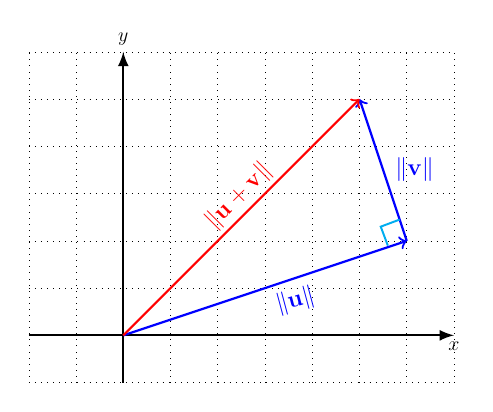
\begin{tikzpicture}[thick,scale=0.6, every node/.style={scale=0.6}]%[scale=.8,font=\scriptsize]
	\draw[help lines,black,dotted] (-2,-1) grid (7,6);
	\draw[thick,-latex] (-2,0) -- (7,0) node[below] {\large $x$};
	\draw[thick,-latex] (0,-1) -- (0,6) node[above] {\large $y$};	
	% vector u
	\draw [color=blue,->] (0,0) -- (6,2);
	%	\fill[color=blue,draw] (4,0.5) node[below,left] {\Large $\mathbf{u}$};
	\fill[color=blue,draw] (2.8,0.5) node[rotate=15,right] {\Large \ \  $\Vert\mathbf{u}\Vert$};
	%	\draw [line width=0.1mm,color=blue,dashed,-] (5,0) -- (5,2);
	%	\fill[color=blue,draw] (5,0) node[below] {\Large $v_1$};
	%	\draw [line width=0.1mm,color=blue,dashed,-] (0,2) -- (5,2);	
	%	\fill[color=blue,draw] (0,2) node[left] {\Large $v_2$};
	% vector v
	\draw [color=blue,->] (6,2) -- (5,5);
	%	\fill[color=blue,draw] (4.8,4.8) node[right] {\Large \ \  $\mathbf{v}$};
	\fill[color=blue,draw] (5.3,3.5) node[rotate=0,right] {\Large \ \  $\Vert\mathbf{v}\Vert$};
	\draw [line width=0.25mm,color=cyan,-] (5.6,1.9) -- (5.45,2.3) -- (5.85,2.45);	
	%	\draw [line width=0.15mm,color=red,dashed,-] (5,2) -- (-4,5);	
	%	\fill[color=red,draw] (1.8,3.5) node[rotate=-20,left] {\Large $d(\mathbf{u}, \mathbf{v})$};
	% vector u+v
	\draw [color=red,->] (0,0) -- (5,5);	
	\fill[color=red,draw] (1.5,2) node[rotate=45,right] {\Large \ \  $\Vert\mathbf{u}+\mathbf{v}\Vert$};
	\end{tikzpicture}
\end{center}

\begin{prop}{\textbf{Propiedad 8 (Teorema de Pitágoras)}}
	\justifying
	Si $\mathbf{u}$ y $\mathbf{v}$ son vectores de $\r^n$, entonces  $\mathbf{u}$ y $\mathbf{v}$ son ortogonales
	si y sólo si
	\[
	\Vert \mathbf{u} + \mathbf{v}\Vert^2 = \Vert \mathbf{u}\Vert^2 + \Vert \mathbf{v}\Vert^2.
	\]
\end{prop}	

\end{frame}
}

%%------------------------------------------------------------------------------------------------------

\subsection{}

{\nologo
\begin{frame}\frametitle{Relación entre el producto punto y el producto de matrices}

\begin{alertblock}{\textbf{Observación 3}}\justifying
	Si los vectores $\mathbf{u}=(u_1,\hdots,u_n) $ y $\mathbf{v}=(v_1,\hdots,v_n)$ de $\r^n$ 
	los representamos como vectores columna
	\[
	\mathbf{u} =
	\left(
	\begin{array}{c}
	u_1\\
	u_2\\
	\vdots \\[1mm]
	u_n
	\end{array}
	\right)\ 
	\qquad \text{y} \qquad 
	\mathbf{v} =
	\left(
	\begin{array}{c}
	v_1\\
	v_2\\
	\vdots \\[1mm]
	v_n
	\end{array}
	\right), 
	\]
	entonces el \textbf{\textit{producto punto}} o \textbf{\textit{producto escalar}} de ellos
	se puede expresar como el producto de matrices
	\[
	\mathbf{u}\cdot \mathbf{v} =
	\mathbf{u}^T \mathbf{v} =
	\left(
	\begin{array}{cccc}
	u_1 & u_2 & \cdots & u_n \\
	\end{array}
	\right) 
	\left(
	\begin{array}{c}
	v_1\\
	v_2\\
	\vdots \\[1mm]
	v_n
	\end{array}
	\right)
	= u_1 v_1 +  \cdots + u_nv_n. 
	\]
\end{alertblock}

\end{frame}
}

%%------------------------------------------------------------------------------------------------------

\subsection{}

{\nologo
\begin{frame}%\frametitle{Relación entre el producto punto y el producto de matrices}

\begin{alertblock}{\textbf{Observación 3}}\justifying
	Si los vectores $\mathbf{u}=(u_1,\hdots,u_n) $ y $\mathbf{v}=(v_1,\hdots,v_n)$ de $\r^n$ 
	los representamos como vectores columna, entonces el \textbf{\textit{producto punto}} o \textbf{\textit{producto escalar}} de ellos
	se puede expresar como el producto de matrices
	\[
	\mathbf{u}\cdot \mathbf{v} =
	\mathbf{u}^T \mathbf{v} =
	\left(
	\begin{array}{cccc}
	u_1 & u_2 & \cdots & u_n \\
	\end{array}
	\right) 
	\left(
	\begin{array}{c}
	v_1\\
	v_2\\
	\vdots \\[1mm]
	v_n
	\end{array}
	\right)
	= u_1 v_1 +  \cdots + u_nv_n. 
	\]
\end{alertblock}

\begin{ej}{\textbf{Ejemplo 9}}
	Calcule el producto punto de los vectores
	\[
	\mathbf{u} =
	\left(
	\begin{array}{r}
	1\\
	2\\
	-1
	\end{array}
	\right)\ 
	\qquad \text{y} \qquad 
	\mathbf{v} =
	\left(
	\begin{array}{r}
	3\\
	-2\\
	4
	\end{array}
	\right). 
	\]	
\end{ej}
\textit{Solución}.

\end{frame}
}

%%------------------------------------------------------------------------------------------------------

\subsection{}

{\nologo
\begin{frame}\frametitle{Proyecciones ortogonales en $\r^n$}

\begin{figure}	
	\begin{subfigure}[b]{0.45\textwidth}
		\centering
		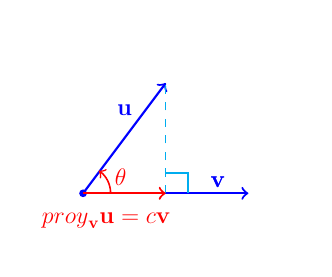
\begin{tikzpicture}[thick,scale=0.7, every node/.style={scale=0.6}]%[scale=.8,font=\scriptsize]
		\draw[help lines,white,dotted] (-1,-1) grid (4,3);
		\fill[color=blue] (0,0) circle[radius=2pt];			
		% Vector u
		\draw [line width=0.27mm,color=blue,->] (0,0) -- (1.5,2);
		\fill[color=blue,draw] (1,1.5) node[below,left] {\Large $\mathbf{u} $};	
		\draw[line width=0.2mm,red,->] (0.5,0) arc (0:55:0.5);
		\fill[color=red,draw] (0.9,0.3) node[left] {\Large $\theta$};
		% Vector v
		\draw [line width=0.27mm,color=blue,->] (0,0) -- (3,0);
		\fill[color=blue,draw] (2.2,0.2) node[below,right] {\Large $\mathbf{v} $};	
		% proy u/v
		\draw [line width=0.15mm,color=cyan,dashed,-] (1.5,0) -- (1.5,2);
		\draw [line width=0.23mm,color=cyan,-] (1.5,0.37) -- (1.9,0.37) -- (1.9,0);
		\draw [line width=0.27mm,color=red,->] (0,0) -- (1.5,0);
		\fill[color=blue,draw] (2.2,0.2) node[below,right] {\Large $\mathbf{v} $};	
		% Valores del ángulo
		\fill[draw] (1.7,-0.5) node[left] {\color{red}\Large $\text{proy}_{\mathbf{v}} \mathbf{u} = c \mathbf{v}$};
%		\fill[draw] (0.5,-1.3) node[left] {\Large $\cos\theta>0$};
		\end{tikzpicture}
		\caption{$c>0$}
	\end{subfigure}
	~ %add desired spacing between images, e. g. ~, \quad, \qquad, \hfill etc. 
	%(or a blank line to force the subfigure onto a new line)
	\begin{subfigure}[b]{0.45\textwidth}
		\centering
		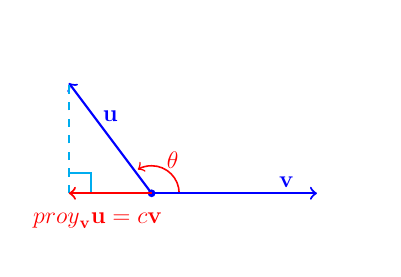
\begin{tikzpicture}[thick,scale=0.7, every node/.style={scale=0.6}]%[scale=.8,font=\scriptsize]
		\draw[help lines,white,dotted] (-2,-1) grid (4,3);
		\fill[color=blue] (0,0) circle[radius=2pt];			
		% Vector u
		\draw [line width=0.27mm,color=blue,->] (0,0) -- (-1.5,2);
		\fill[color=blue,draw] (-0.5,1.4) node[below,left] {\Large $\mathbf{u} $};	
		\draw[line width=0.2mm,red,->] (0.5,0) arc (0:120:0.5);
		\fill[color=red,draw] (0.6,0.6) node[left] {\Large $\theta$};
		% Vector v
		\draw [line width=0.27mm,color=blue,->] (0,0) -- (3,0);
		\fill[color=blue,draw] (2.2,0.2) node[below,right] {\Large $\mathbf{v} $};	
%		\fill[color=blue,draw] (2.2,0.2) node[below,right] {\Large $\mathbf{v} $};	
		% proy u/v
		\draw [line width=0.15mm,color=cyan,dashed,-] (-1.5,0) -- (-1.5,2);
		\draw [line width=0.23mm,color=cyan,-] (-1.5,0.37) -- (-1.1,0.37) -- (-1.1,0);
		\draw [line width=0.27mm,color=red,->] (0,0) -- (-1.5,0);		
		% Caption
		\fill[draw] (0.3,-0.5) node[left] {\color{red}\Large $\text{proy}_{\mathbf{v}} \mathbf{u} = c \mathbf{v}$};
		%		\fill[draw] (0.5,-1.3) node[left] {\Large $\cos\theta>0$};
		\end{tikzpicture}
		\caption{$c<0$}
	\end{subfigure}
	%	\caption{Pictures of animals}\label{fig:animals}
\end{figure}

\begin{defi}{\textbf{Definición 6}}\justifying
	\justifying
	Sean $\mathbf{u}$ y $\mathbf{v}$ vectores no nulos de $\r^n$. La \textbf{\textit{proyección ortogonal}} de $\mathbf{u}$ sobre $\mathbf{v}$
	es el vector definido por
	\[
		\text{proy}_{\mathbf{v}} \mathbf{u} = \frac{\mathbf{u}\cdot \mathbf{v}}{\Vert \mathbf{v}\Vert^2}\ \mathbf{v}
	\]
\end{defi}	

\end{frame}
}

%%------------------------------------------------------------------------------------------------------

\subsection{}

\begin{frame}\frametitle{Proyecciones ortogonales en $\r^n$}

\begin{defi}{\textbf{Definición 6}}\justifying
	\justifying
	Sean $\mathbf{u}$ y $\mathbf{v}$ vectores no nulos de $\r^n$. La \textbf{\textit{proyección ortogonal}} de $\mathbf{u}$ sobre $\mathbf{v}$
	es el vector definido por
	\[
	\text{proy}_{\mathbf{v}} \mathbf{u} = \frac{\mathbf{u}\cdot \mathbf{v}}{\Vert \mathbf{v}\Vert^2}\ \mathbf{v}
	\]
\end{defi}	

\begin{ej}{\textbf{Ejemplo 10}}
	Encuentre la proyección ortogonal de $\mathbf{u}=(6,2,4)$ sobre $\mathbf{v}=(1,2,0)$.
\end{ej}
\textit{Solución}.

\end{frame}
